%__________________________________________________________________________________________ %
%-------------------------------------------PFC---------------------------------------------%
%__________________________________________________________________________________________ %


%%%%%%%%%%%%%%%%%%%%%%%%%%%%%%  PREAMBULO  %%%%%%%%%%%%%%%%%%%%%%%%%%%%%%%%%%%%%
% ----------------------Especificaciones de dise�o---------------------------- %

\NeedsTeXFormat{LaTeX2e}
\documentclass[12pt]{book}

\usepackage{a4}
\usepackage[Lenny]{fncychap}    % Estilos para capitulos
\usepackage{fancyhdr}           % Estilos para cabeceras
%\usepackage[spanish]{babel}
%usepackage[latin1]{inputenc}

% Para no tener problemas con las tildes
\usepackage[utf8]{inputenc}
\usepackage[spanish]{babel}

\usepackage{epsfig}
\usepackage{subfig}
\usepackage{epstopdf}
\usepackage{caption}
\usepackage{keyval}
\usepackage{graphicx}
\usepackage{float}              % Para poner las imags en cualquier sitio
\usepackage{listings}
\usepackage{color}
\usepackage{textcomp}
\usepackage{verbatim}
\usepackage{exceltex}



\definecolor{listinggray}{gray}{0.98}
\definecolor{lbcolor}{rgb}{0.98,0.98,0.98}
\lstset{
	backgroundcolor=\color{lbcolor},
	tabsize=3,
	rulecolor=,
	language=matlab,
	basicstyle=\footnotesize\sffamily,
	aboveskip={1.5\baselineskip},
	belowskip={1.5\baselineskip},
	columns=fixed,
	showstringspaces=false,
	extendedchars=true,
	breaklines=true,
	prebreak = \raisebox{5ex}[5ex][5ex]{\ensuremath{\hookleftarrow}},
	frame=none,
	showtabs=false,
	showspaces=false,
	showstringspaces=false,
	identifierstyle=\ttfamily,
	keywordstyle=\color[rgb]{0,0,1},
	commentstyle=\color[rgb]{0.133,0.545,0.133},
	stringstyle=\color[rgb]{0.627,0.126,0.941},
}

\usepackage[numbers,sort&compress,comma]{natbib}	% Modo de poner la bibliograf�a
\usepackage{verbatim}      %  \begin{comment}...\end{comment}
\usepackage{subeqnarray}   % equationarray with numbers 1a, 1b, ...
\usepackage{bbm}           % Para s�mbolo tipo n�meros reales. Ej: \bbm{R}
\usepackage{longtable}     % Para tablas largas de m�s de una p�gina
\usepackage{rotating}
\usepackage{psfrag}        % Para cambiar fragmentos de text en .eps por otro en latex
\usepackage{pifont}        % Para otros s�mbolos
\usepackage{fancybox}      % Para encuadrar texto en recuadros
\usepackage{amsmath}       % Mejora la calidad de las formulas
\usepackage{amsfonts}
\usepackage [linktocpage]{hyperref}      % Para enlaces de hipertexto
\usepackage{amssymb,amsfonts}
\usepackage{multirow}
\usepackage{booktabs}
\usepackage{color}
\usepackage{longtable}
\usepackage{float}
\usepackage{array}




\setcounter{tocdepth}{2}             % toc = table of contents. Para definir niveles del �ndice
\setcounter{secnumdepth}{5}          % Hasta cu�ndo se enumeran los caps, seccs, etc


\setlength{\topmargin}{-1.1cm}        % margen por arriba
\setlength{\parskip}{\baselineskip}
\setlength{\parskip}{0.3cm}          % Espacio entre parrafos
\setlength{\textwidth}{16.5cm}       % Ancho del �rea imprimible	
\setlength{\evensidemargin}{-0.4cm}  % Margen izdo en p�ginas pares
\setlength{\oddsidemargin}{0.3cm}    % Margen izdo en p�ginas impares
% evensidemargin = -oddsidemargin !!!

\setlength{\headsep}{1.0cm}
\setlength{\headheight}{3ex}
\setlength{\footnotesep}{5mm}
%\setlength{\mathindent}{1.0cm}       % Controla el espacio entre margen y ec si no est� centrada


%%% Definitionen f�r Fancy Headings
%\renewcommand{\baselinestretch}{3mm}
%\renewcommand{\labelenumi}{\roman{enumi}.}
%\renewcommand{\chaptermark}[1]{\markboth{#1}{}}
%\renewcommand{\sectionmark}[1]{\markright{\thesection\ #1}{}}
\renewcommand{\labelitemi}{$\bullet$}
\renewcommand{\labelitemii}{$\diamond$}
\renewcommand{\labelitemiii}{$\cdot$}

\lhead[\fancyplain{}{\thepage}]{\fancyplain{}{\sl\nouppercase\rightmark}}
\rhead[\fancyplain{}{\sl\nouppercase\leftmark}]{\fancyplain{}{\thepage}}
\cfoot{}
\pagestyle{fancyplain}  		% normale Kopfzeile; ohne Seitenzahl: empty

% Formato de capitulos
\ChTitleVar{\sf\Huge} % Tama�o de la letra del nombre del cap
\ChTitleAsIs


%%% Comando para quitar encabezado y pie de las pag en blanco
\newcommand{\clearemptydoublepage}
{\newpage{\pagestyle{empty}\cleardoublepage}}

\newcommand{\R}{\mathbb{R}}
\newcommand{\x}{\mathbf{x}}
\newcommand{\grad}{\hspace{-2mm}$\phantom{a}^{\circ}$} %para los grados centigrados

%%% Abstract
\newenvironment{abstract}
{\begin{center}
		\begin{minipage}{0.8\textwidth}
			\slshape}
		{\end{minipage}
	\end{center}}
	
	
	\typeout{ }
	\typeout{----------------------------------------------------------------------}
	\typeout{ }
	
	



%%%%%%%%%%%%%%%%%%%%%%%%%%%%%%  DOCUMENTO  %%%%%%%%%%%%%%%%%%%%%%%%%%%%%%%%%%%%%
%-------------------------Cuerpo del documento---------------------------------%


\begin{document}
	\renewcommand{\contentsname}{Contents}
	\renewcommand{\listfigurename}{List of figures}
	\renewcommand{\listtablename}{List of tables}
	\pagenumbering{roman}    % Numeraci�n de p�ginas con num romanos
	\setcounter{page}{1}      % Establece la siguiente p�gina como la 1
	\begin{titlepage}
\label{ch:portada}
\begin{center}

{\Large\textsc{Ingenier�a de Telecomunicaci�n}}


Departamentos:  \\ Arquitectura y Tecnolog�a de Computadores \\ Teor�a de la Se�al, Telem�tica y Comunicaciones

\textbf{Universidad de Granada}


\vspace{0.5cm}

\begin{figure}[h]
	\centering
	\epsfig{file=figuras/Portada/portada1, width=7cm}
	\label{fig:ugr}
\end{figure}


\vspace{0.5cm}
\textbf{PROYECTO FIN DE CARRERA}


\vspace{0.9cm}


{\Huge\textbf{Desarrollo de una aplicaci�n de visualizaci�n de datos y configuraci�n para sistemas de monitorizaci�n y an�lisis del movimiento del cuerpo humano.}}


\end{center}


\vspace{1.5cm}
\textbf{Realizado por:}  \hfill \textbf{Dirigido por:}

Javier L�pez Garc�a \hfill D. Alberto Olivares Vicente

\hfill D. Gonzalo Olivares Ruiz

\end{titlepage}
		% Inclu�mos la portada en espa�ol
	\clearemptydoublepage
	
	%Declaración
%--------

\begin{titlepage}
\label{ch:Statement}
\vspace{2cm}

\noindent  D. Alberto Olivares Vicente, profesor  del dpto. de Teoría de la Señal, Telemática y Comunicaciones, como director del Proyecto Fin de Carrera de Dª. Verónica Torres Sánchez,

\vspace{2cm}
\noindent Informan:

\vspace{1.5cm}
\noindent Que el presente trabajo, titulado:

\noindent \textbf{Comparison of Posturographic Body-sway Measurements with Inertial Data of Parkinson Patients.}

\noindent Ha sido realizado y redactado por el mencionado alumno bajo nuestra dirección, y con esta fecha autorizamos a su presentación.
\vspace{3.5cm}

\noindent Granada, a 20 de julio de 2015 Fdo:

\vspace{6.5cm}
\noindent D. Alberto Olivares Vicente    \hfill   D. Juan Manuel Górriz Sáez

\end{titlepage}       % Incluimos la declaración del proyecto
	\clearemptydoublepage
	\begin{titlepage}
\label{ch:acknowledgements}
{ \huge \bfseries Acknowledgements \\[0.4cm] }


First and foremost, I would like to thank Dr Alberto Olivares Vicente and Juan Manuel Górriz Sáez for supervising this work, his assistance and most especially for his continuous motivation and encouragement.

Thanks to Robin Weiss for his suggestions, his great ideas and knowledge, his jokes when the work was being  hard and, in short, for helping me along this Project.

Special thanks go to my friends for valuing my work, encouraging me every day, their advices and making me smile with their crazy things. Of course, many thanks go to my friend and flatmate, for putting up with me in the work nights and making to laugh with their positive music .

Finally, I am deeply grateful to my family, for giving me the opportunity to study, respecting all my decisions and their motivation and affection.


\end{titlepage}       % Incluimos agradecimientos
	\clearemptydoublepage
	\begin{titlepage}
\label{ch:abstract}
{ \huge \bfseries Abstract \\[0.4cm] }

\end{titlepage}       % Incluimos resumen
	\clearemptydoublepage
	
\begin{titlepage}
\label{ch:abbrevations}
{ \huge \bfseries Abbrevations \\[0.4cm] }

\textbf{APA}: Anticipatory postural adjustments

\textbf{SIPBA}: Signal processing and Biomedical Applications

\textbf{FP}: force plate

\textbf{GW}: Gait Watch

\textbf{QS}: Qualysis System

\textbf{PD}: Parkinson’s disease

\textbf{IMU}: Inertial Measurement Unit

\textbf{MIMU}: Magnetic Inertial Measurement Unit

\textbf{EMG}: Electromyography

\textbf{MEMS}: Microelectromechanical Systems

\textbf{LTSD}: Long Term Spectral Detector

\textbf{FSD}: Framed Spectrum Detector

\textbf{COP}: center of pressure

\textbf{AP}: Antero-posterior

\textbf{ML}: Medio Lateral

\textbf{FIR}: Finite Impulse Response.


\end{titlepage}       % Incluimos abreviaciones
	\clearemptydoublepage
	
	\tableofcontents          % Pone índice
   \listoffigures		   	% Crea la lista de figuras
   \listoftables			% Crea la lista de tablas
	\clearemptydoublepage

	

	\clearemptydoublepage
	\include{Introduccion}
	\clearemptydoublepage
	\chapter{Hardware Description}
\label{ch:Hardware}
Along this chapter we will introduce a general description of all devices used to data gathering for the development of this project.


It should be noted at this point that there are two clearly differentiated parts. In the first of them, we work with Force Plate and GaitWatch data, taking out their characteristic signals and synchronising them. In the second of them, we work jointly with Gait Watch and Qualisys System data for the purpose of comparing the accuracy in the calculated orientation angles.


\section{GaitWatch}

GaitWatch is an Inertial Measurement Unit (IMU) designed for gait monitoring of patients. It was developed by Prof. Dr. Med. Kai B¨otzel at the Department of Neurology of Ludwig-Maximilians University in Munich in conjunction with Dr. Alberto Olivares Vicente from the Department of Signal Theory, Telematics and Communications of the University of Granada. \cite{OlivaresBotzel2013}

The system is composed of the central processing unit and
a set of measuring units which are wired to it. The measuring units are 
placed in the patients’ thighs, shanks, arms and trunk.

The central processing unit has a microcontroller is in charge of gathering the data from the external measurement units and writing it to the memory card. So, this central unit is placed in the trunk inside a box and it contains an AL-XAVRB board with an AVRATxmega processor which contains the necessary embedded firmware to gather the data from all the measurement units and store it in a microSD card. Also, the trunk box contains some embedded magnetic and inertial sensors.

There are three different kinds of external units with the following components:
\begin{itemize}
	\item Type A (thighs and shanks): 
	\begin{itemize}
		\item IMU 5 from Sparkfun. IMU 5 contains an IDG500  biaxial gyroscope (from which only Y axis is actually used) with a measurement range of $\pm500deg/s$ and a $\pm3g$ triaxial accelerometer, ADXL335 .
	\end{itemize}
	\item Type B (arms):
	\begin{itemize}
		\item IDG500  biaxial $\pm500deg/s$ gyroscope.
	\end{itemize}
	\item Type C (trunk box):
	\begin{itemize}
		\item ADXL345  triaxial accelerometer with programmable range ($\pm16g/\pm8g/\pm4g/\pm2g$).
		\item IMU3000 triaxial gyroscope with programmable range ($\pm250/\pm500/\pm1000/\pm3000 (deg/s)$).
		\item Micromag3  triaxial magnetometer ($\pm11Gauss$).
	\end{itemize}
\end{itemize}


\section{Force Platform}

\section{Qualisys System}
	\clearemptydoublepage
	\chapter{Synchronisation}
\label{ch:Synchronisation}

\section{Introduction and chapter's structure}
One of the most important aspects whether you have data acquired from multiples devices or channels is the synchronisation. If these data are not appropriately correlated or synchronised, the analysis and conclusions from your use will be erroneous. Also, it’s very important doing all automatically when you have a data on a broad scale.
Therefore, the following sections explain how the information has been obtained and processed automatically, as well as what features have been calculated to characterise the movements of the patients and to carry out the synchronisation between the Force Plate signals and GaitWatch signals. This content is superficially depicted in figure XX.

\begin{figure}[H]
	\centering
	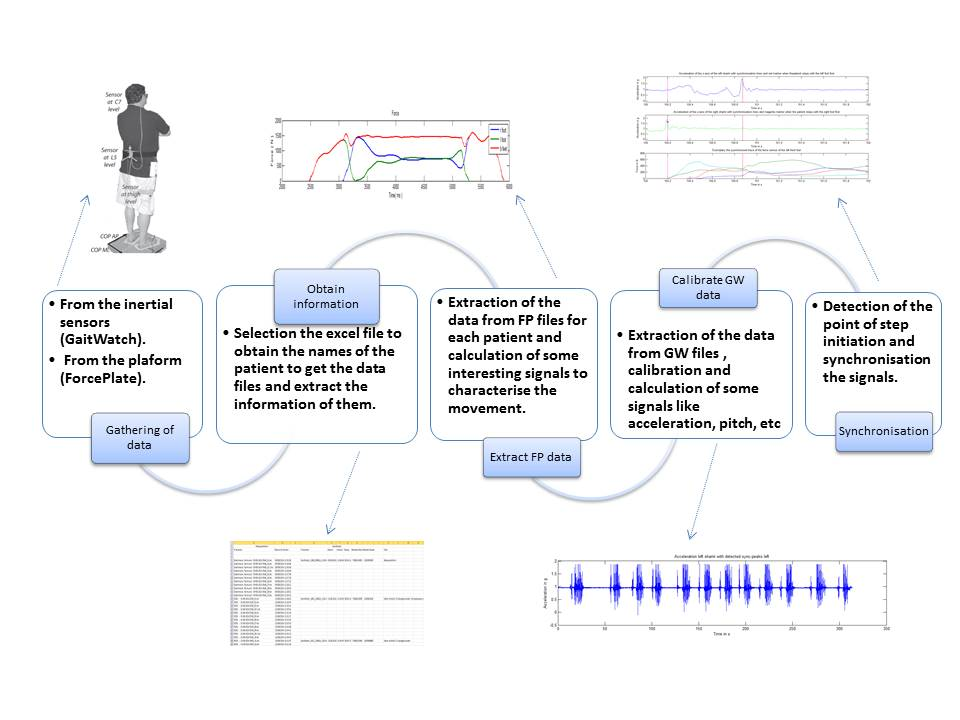
\epsfig{file=imagenes/diagramSynchronisation, width=7cm}
	\caption{Diagram of the Synchronisation's progress.}
	\label{fig:arte1}
\end{figure}

\section{Data gathering Protocol}
Prior to start of data gathering, it’s necessary to set up the protocol for procedure that patients have to carry out while the data are recorded. The establishing this procedure is very important so that the synchronisation works properly because we have to identify a clear movement in both signals to match one signal with the other at the same time.
In addition, the realised movements must be representatives to obtain conclusive data which help us to extract characteristics for the purpose of identify differences between patients and control subjects subsequently.

The steps followed by the patients are detailed hereafter:

1.	Subject stands in front of the Force Plate.

2.	Gait watch record starts for data gathering.

3.	Force plate record starts for data gathering.

4.	Subject makes a step onto the platform.

5.	Subject stands on the platform a variable time between 2 and 10 seconds.

6.	Subject makes some step  forward and turns left to stand in front of the platform again.

This procedure is repeated ten times by each subject in order to characterise better the movement made.
It’s important to clarify that the GaitWatch recording contains all these ten episodes ( in other cases more) and the platform recording only contains one episode each. So, this is a fact that we have to consider to do the synchronisation.


\section{Design of developed code  in Matlab}
	\subsection{Selection, reading and obtaining of information from the excel file}
	\subsection{Extraction of the forceplate data}
	\subsection{Calibration of the GaitWatch data}
	\subsection{Synchronisation}	
\section{Results discurssion}		

	
	\clearemptydoublepage
	\bibliographystyle{unsrt}
	\bibliography{biblio}
	
	\clearemptydoublepage
\end{document}